\section{Introduction} \label{sec:i}

Connectomics---reconstructing the wiring diagram of a mammalian brain at nanometer resolution---results in datasets at the scale of petabytes~\cite{suissapeleg2016,haehn_dojo_2014}. Machine learning methods find cell membranes and create cell body labelings for every neuron~\cite{ronneberger2015u,liu2014modular,GALA2014} (Fig.~\ref{fig:data}).
%aims to reconstruct the wiring diagram of a mammalian brain at nanometer resolution. This results in datasets at the scale of petabytes~\cite{suissapeleg2016}. 
%These shear amounts of data require sophisticated methods of compression to enable efficient storage and transfer. 
These segmentations are stored as label volumes that are typically encoded in 32 bits or 64 bits per voxel to support labeling of millions of different nerve cells (neurons).  Storing such data is expensive and transferring the data is slow. To cut costs and delays, we need compression methods to reduce data sizes.

%Our work stems from a collaboration between computer scientists and neuroscientists in the field of connectomics. 
%Connectomics aims to reconstruct the wiring diagram of a mammalian brain at nanometer resolution, comprising millions of nerve cells (neurons) and their interconnections. 
%By deciphering this vast network and analyzing its underlying properties, scientists hope to better understand mental illnesses, learning disorders, and neural pathologies.

\begin{figure}[h]
	\begin{center}
		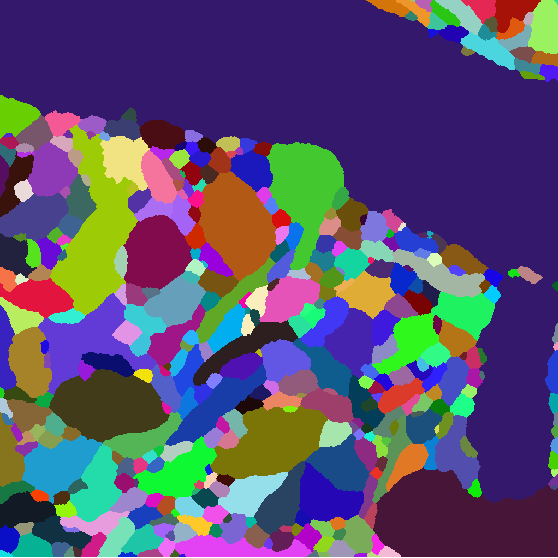
\includegraphics[width=0.38\textwidth]{gfx/ac3.png}%
		\hspace{0.12\textwidth}
		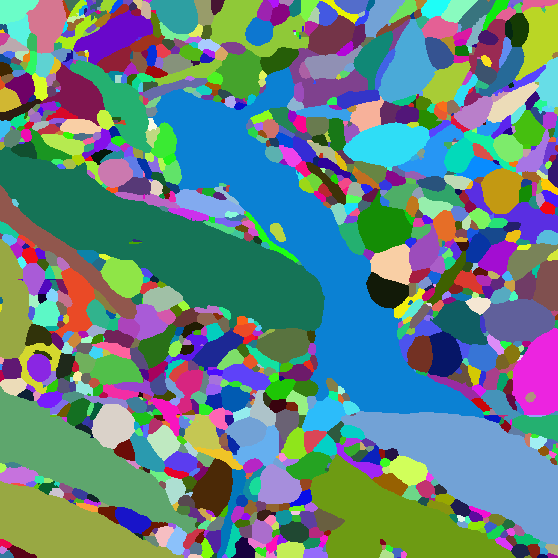
\includegraphics[width=0.38\textwidth]{gfx/cyl.png}%
	\end{center}
\caption{Examples of connectomics segmentation data with a different color per cell.}
\label{fig:data}
\end{figure}

%To analyze neuronal connectivity at the level of individual connections of neurons, we acquire and process high-resolution electron microscopy (EM) image stacks. 
%Recent progress in automatic sample preparation and EM acquisition techniques increases these datasets to petabytes in size~\cite{suissapeleg2016}.
%Machine learning methods find cell membranes and create cell body labelings for every neuron~\cite{ronneberger2015u,liu2014modular,GALA2014} (Fig.~\ref{fig:data}). 
%These segmentations are stored as label volumes, which are typically encoded in 32 bits or 64 bits per voxel to support millions of unique labels. 
%Storing such data is costly, and transferring the data is slow. To cut costs and delays, we need compression methods to reduce data sizes.

%One approach to allow data analysis of these volumes is to pre-process the segmentation data and store it uncompressed as a tiled quadtree data structure on a network filesystem.
%Researchers then access the segmentation data with thin clients, e.g., web-based applications like Dojo~\cite{haehn_dojo_2014}.
%The quadtree structure represents different pre-computed zoom levels of the data and enables loading and exploration of downsampled images.
%This scenario imposes three problems: offline storage, data transmission, and random access.
%Currently, the complete dataset is stored on disk and only a subset is transferred depending on individual use cases. This works well; however, recent progress in automatic sample preparation and EM acquisition techniques increases connectomics data to terabytes in size~\cite{RonnebergerFB15,GALA2014}. Storage and transmission of such massive datasets is hard and expensive, and access can be slow. Therefore, we need compression methods to reduce data sizes.

The literature currently lacks efficient compression of label volumes. 
General-purpose compression schemes~\cite{deutsch1996zlib,ziv1978compression,lehmann2016liblzf,oberhumer2005lzo,welch1984technique,seward1998bzip2,pavlov2007lzma,vandevenne2016zopfli,google2016brotli,collet2016smaller} are not optimized for this data.
In this paper, we exploit the typical characteristics of label volumes such as large invariant regions without natural relationship between label values. 
These properties render 2D image compression schemes inadequate since they rely on frequency reduction (using e.g., wavelet or discrete cosine transform) and value prediction of pixels based on local context (differential pulse-code modulation)~\cite{roelofs1999png,skodras2001jpeg}. 
Color space optimization strategies in video codecs~\cite{aimar2005x264} also have no effect on label volumes, even though the spatial properties of a segmentation stack (\textit{z}-axis) are similar to the temporal properties of video data (time-axis). 
A compression scheme designed specifically for label volumes is part of the visualization software Neuroglancer~\cite{google2016compressed}. 
This method exploits segmentation homogeneity by creating small blocks with $N$ labels and reducing local entropy to $\log_2{N}$ per pixel. 
Lookup tables then decode the values $[0,N)$ to the original 64-bit labels. We compare the Neuroglancer scheme with our method.
%The most relevant current compression tool is Neuroglancer~\cite{google2016compressed}---a web-based 3D segmentation viewer that provides a compression scheme for segmentation data.
%
%The assumption behind this scheme is that, on average, small local areas will contain very few unique labels with high probability. Based on this assumption, Neuroglancer divides the segmentation data into several small blocks. Pixels inside a block with $N$ distinct labels only require $\log_2{N}$ bits of information to encode.
%
%A lookup table for each block maps the values $[0, N)$ to the original 64-bit label. We compare the performance of Neuroglancer with our scheme in Sec.~\ref{sec:results}.
%
%A compression scheme for labeled volumes is part of the 3D segmentation viewer Neuroglancer~\cite{google2016compressed}. This method exploits segmentation homogeneity by creating small blocks with $N$ labels, reducing entropy to $\log_2{N}$. Lookup tables map the values $[0,N)$ to the original 64-bit labels. We compare the performance of Neuroglancer with our scheme in Sec.~\ref{sec:results}.
%
%and therefor reduces the
%to exploit homogeneity
%
%The most relevant current compression is

We explore the lossless compression of gigavoxel neuron segmentation volumes with high bit-encodings. 
We study and evaluate the performance of existing lossless compression methods, and their combinations, on multiple connectomics, magnetic resonance imaging (MRI) and general segmentation datasets.
As our main contribution, we present \appName---a novel compression method designed for label volumes using windowed feature extraction. 
\appName yields compression ratios on label volumes 80\% higher than the current best tools (Sec.~\ref{sec:results}).
We release an open-source C++ implementation of our method including a Python interface.
